\chapter*{Zeitmanagement}
	\documentPartEntry{Zeitmanagement}
	Zur zeitlichen Planung und für die Auswertung der Arbeitszeit haben wir das \ppt\ Jira\footnote{\url{https://de.atlassian.com/software/jira}} verwendet,
	wie wir es auch für das ganze Projektmanagement verwendet haben.
	Zu jedem neu erstellten Task haben wir auch die zur Umsetzung geschätzte Dauer erfasst.
	Gleichzeitig haben wir auch die effektive benötigte Zeit gebucht.
	Ein Beispiel für eine Erfassung von Arbeitszeit ist in Abbildung~\ref{fig:logWork} abgebildet.
	
	\begin{figure}[H]
		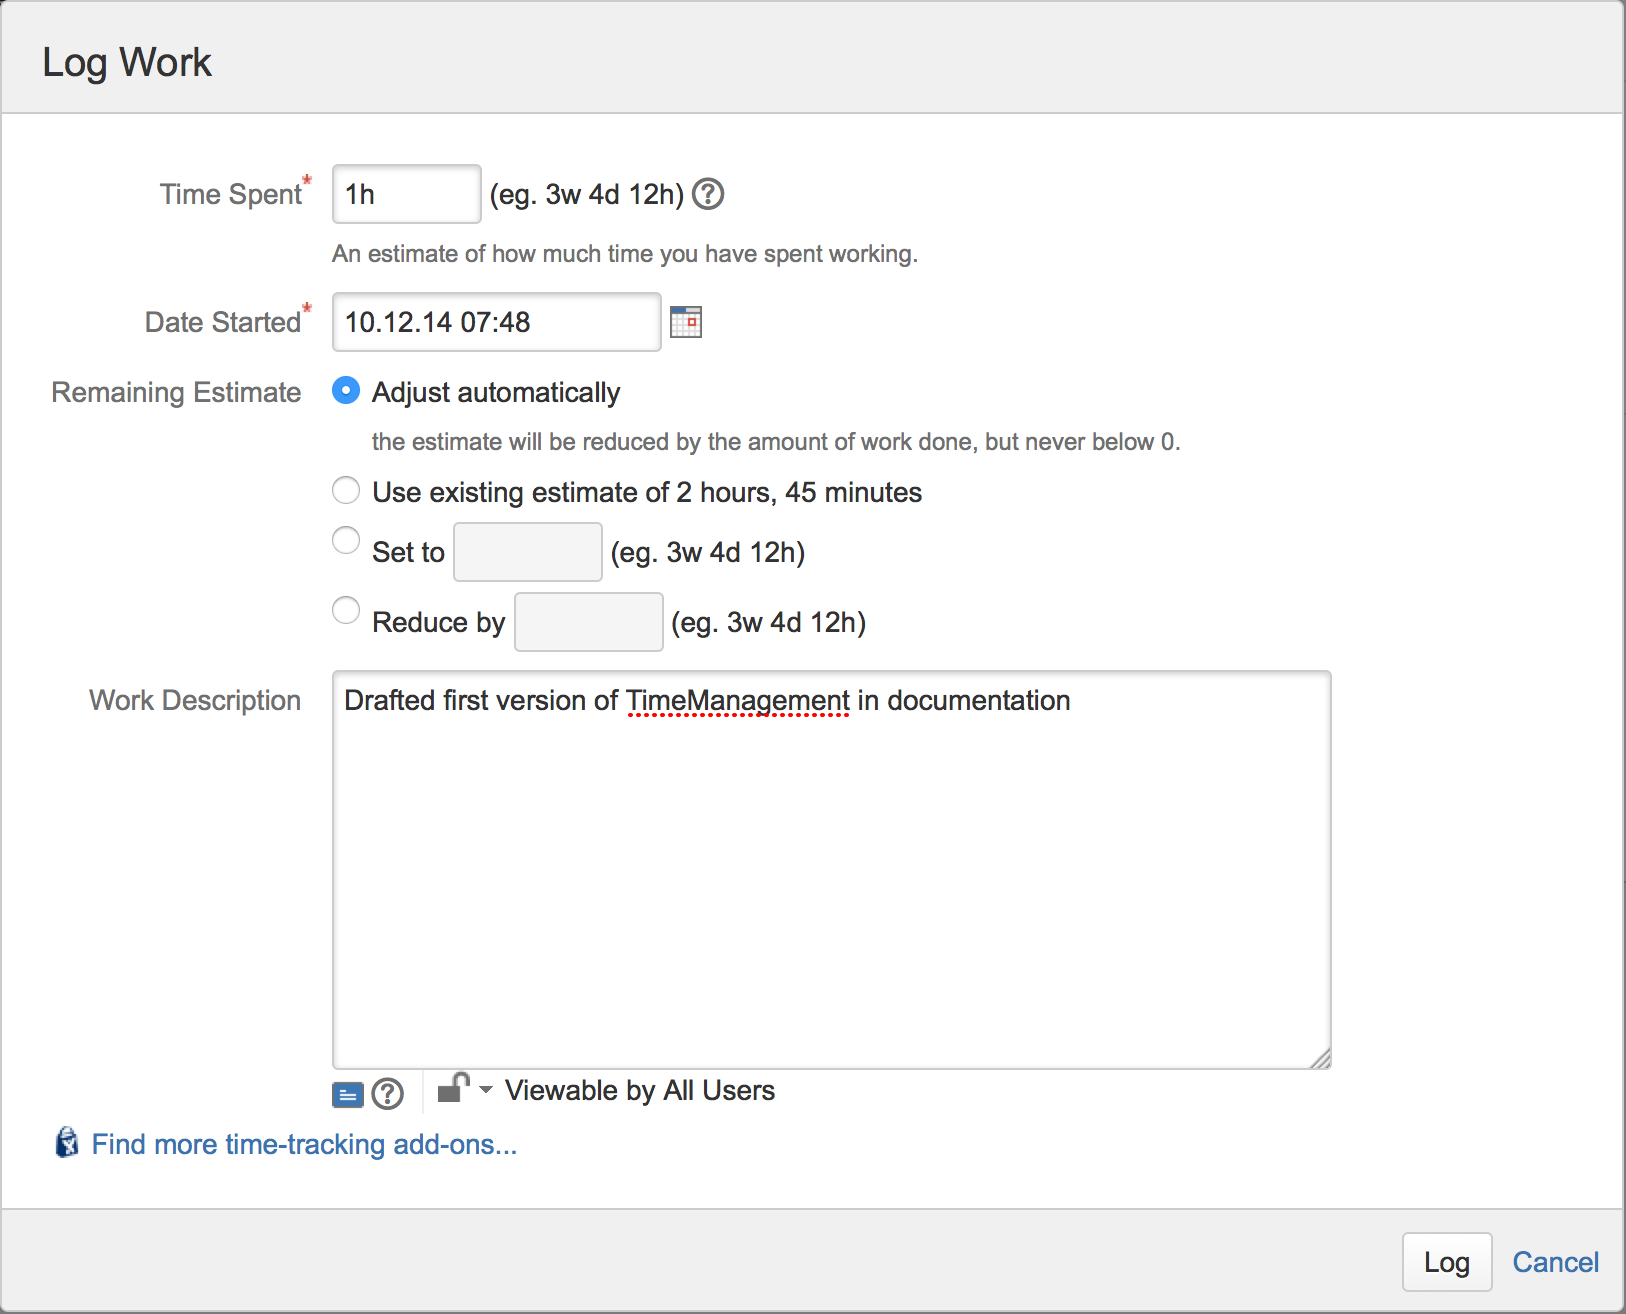
\includegraphics[width=0.8\textwidth]{projectPlan/media/img/logWork.png}
		\centering
		\caption{Erfassen von Arbeitszeit im Jira}
		\label{fig:logWork}
	\end{figure}
	
	Die erfassten Arbeitszeiten haben wir mit einem eigenen Ruby-Skript über die REST-API von Jira\footnote{\url{https://docs.atlassian.com/jira/REST/latest/}} exportiert
	und in einer Excel-Tabelle laufend ausgewertet.
	Grund dafür ist die dazu fehlende Funktion im Basispaket von Jira\footnote{Es gibt eine kostenpflichtige Erweiterung, die Reporting anbietet}.
	
	Entstanden ist folgender Graph der geleisteten Arbeit in Abbildung~\ref{fig:workGraph}.
	Er zeigt den kontinuierlichen Verlauf während dem Projekt
	und die ausgeglichene Arbeitslast zwischen Tobias Blaser und Laurin Murer.
	Bereits von Anfang der Projektplanung an war geplant, die Arbeit eine Woche vor offiziellem Abgabetermin fertig zu stellen, um genügend Pufferzeit zu besitzen und ohne Stress drucken und abgeben zu können.
	
	Diese Planung hat sich sehr bewährt, die Arbeit wurde mit dem kleinen aber geplanten Schlussspurt wie vorgesehen fertig.
	Da geplant war, die Arbeit früher fertig zu stellen, endet die Linie des Soll-Max in Abbildung~\ref{fig:workGraph} auch zu dieser Zeit.
	Die beiden Soll-Linien geben die von der HSR vorgegebene\footnote{Siehe Aufgabenstellung} minimal und maximal erwarteten Aufwände an.
	
	\begin{figure}[H]
		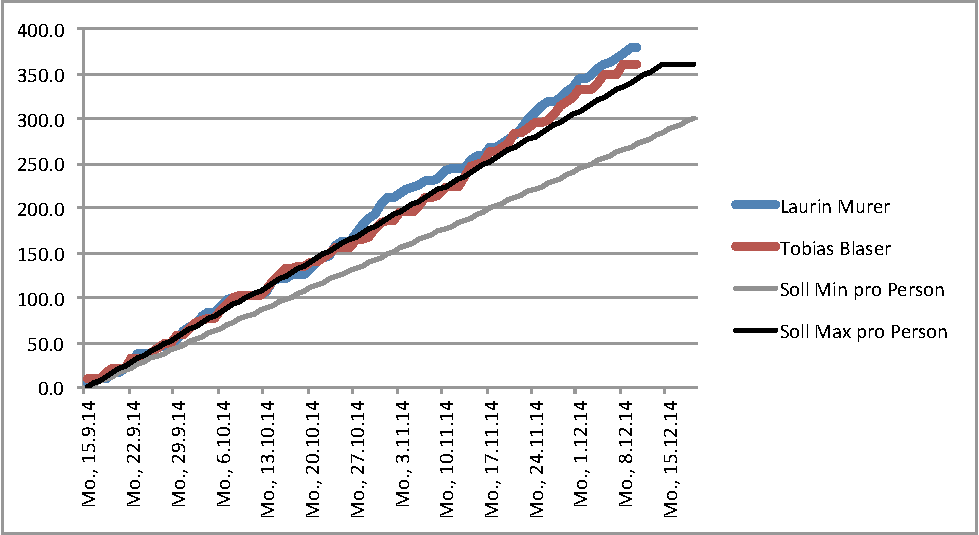
\includegraphics[width=\textwidth]{projectPlan/media/img/workGraph.pdf}
		\centering
		\caption{Graph über die geleistete Arbeit}
		\label{fig:workGraph}
	\end{figure}
	
	Wir haben von Begin des Projektes geplant, viel in das Projekt zu investieren, um ein sehr gutes Ergebnis zu erreichen.
	
	Die gleichmässig steigenden Graphen zeigen, dass sich unsere Projektplanung bewährt hat.
	
	In Abbildung~\ref{fig:weekhours} werden die Arbeitsstunden pro Woche ausgewiesen.
	Hier zeigt sich nochmals die Kontinuität über das gesamte Projekt.
	Kurzzeitig gibt es Schwankungen, die jedoch zeitnah wieder ausgeglichen werden.
	Die grösseren kurzfristigen Schwankungen sind auf Aktivitäten ausserhalb der Bachelorarbeit zurückzuführen,
	wie beispielsweise einen beruflichen Messebesuch in Berlin oder Überzeitkompensation im Büro,
	sowie auf den Schluss\-effort.

	\begin{figure}[H]
		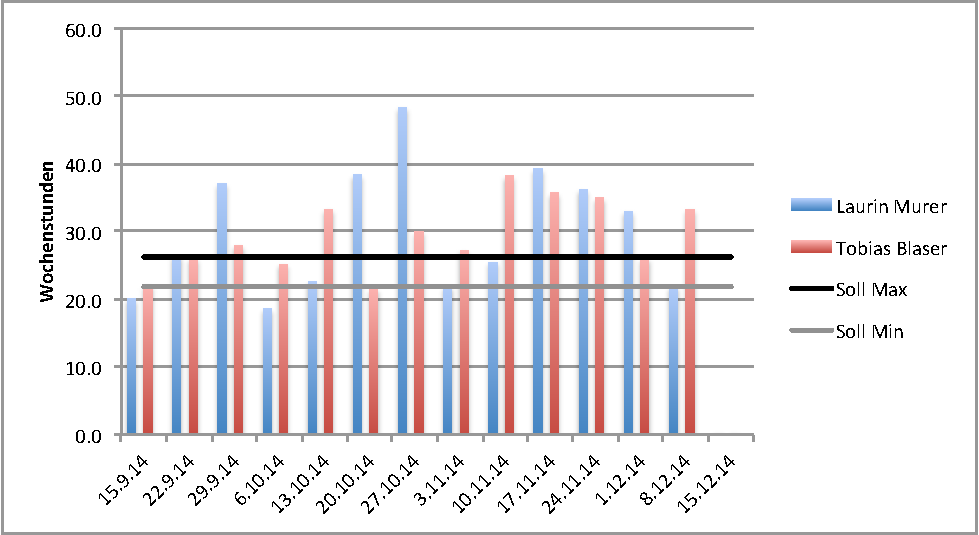
\includegraphics[width=\textwidth]{projectPlan/media/img/weekhours.pdf}
		\centering
		\caption{Graph über die geleistete Arbeit pro Woche}
		\label{fig:weekhours}
	\end{figure}

	\subsection*{Schätzgenauigkeit der Aufwände}
	Wenig verwunderlich liegt die Schätzgenauigkeit bei kleinen Paketen nahe der effektiv benötigten Zeit.
	Bei grösseren Paketen ist die Differenz grösser und schwankt zwischen 50\% weniger und 100\% mehr benötigte Zeit als Extremwerte.
	Wir haben dabei häufiger den Aufwand überschätzt als unterschätzt.
	Nach Hochrechnungen liegt die durchschnittlich geschätzte Dauer zwischen 80\% und 100\% der effektiv benötigten Zeit.
	
	In dieser Rechnung nicht mit eingeschlossen sind neu erstellte Issues aufgrund der Notwendigkeit der Umsetzung weiterer Teilaspekte eines grösseren Issueblocks.
	Würde man dies mitberücksichtigen, so liegt die effektiv benötigte Zeit schätzungsweise zwischen 20\% und 40\% über der geschätzten Zeit.
	Aufgrund dieser Erkenntnis in den ersten Wochen haben wir für die restlichen Meilensteine jeweils maximal 2/3 der Zeit für Features eingeplant
	und die restliche Zeit einerseits für administrative Tätigkeiten und andererseits als Puffer vorgesehen, was sich bewährt hat. 
